\chapter{Variations d'implémentation et mesures de performance}\label{perf_chap}

Les chaînes de caractères étant des structures de données, il existe
plusieurs façons de les implémenter, chacune avec ses avantages
et ses inconvénients.

Au delà même de la structure de base, des variations existent dans
la gestion en interne de ces structures, choix qui auront un impact
sur les opérations primitives de la structure et par extension sur
l'ensemble des services.

Les variations ont ici lieu à plusieurs niveaux:

\begin{enumerate}
	\item Au niveau de la complexité algorithmique
	\item Au niveau de l'affinité des processeurs avec les structures de données
\end{enumerate}

Nous souhaitons mettre l'accent sur la deuxième partie des optimisations,
qui est la plus importante dans notre cas.
En effet, notre solution ayant pour but d'être utilisée par les programmeurs,
il est important de veiller à ce que sa performance soit maximale dans le
cas de programmes réels, et non seulement dans le cas de benchmarks.

Ce chapitre énumère et les compare des variations d'implémentations par le biais
de benchmarks sur des programmes existants et sur des cas basiques.
Nous montrons via ces programmes de mesure que notre
approche mélangeant cordes et chaînes plates est aussi performante que les
implémentations à chaînes plates dans des cas d'utilisation réels, tout en
permettant d'éviter les cas dégénératifs exposés par celles-ci.

Nous allons séparer les validations en deux parties; une première sur
des micro benchmarks, servant à mettre en exergue les capacités de la
solution à résister aux cas dégénératifs d'utilisation de chaînes de
caractères; et une deuxième partie qui consistera à l'utilisation de
notre modèle sur des programmes réels et à comparer la performance par
rapport à d'autres programmes équivalents dans d'autres langages.

\section{Protocole expérimental}

Chaque benchmark de la suite est exécuté sur un ordinateur fixe possèdant un processeur
64-bit Intel i5-4670 @3.40 GHz, 8Gio de mémoire vive de type DDR3-1600 utilisant un système
d'exploitation Linux Mint 17.2-Rafaela, avec un noyau 3.16.0-38-generic.

Chaque benchmark est exécuté 5 fois, le temps moyen est retenu pour inclusion
dans les résultats.
Le temps d'exécution est mesuré à l'aide de GNU time, seul le temps utilisateur est pris
en compte.

\section{Représentativité de Nit}

Dans cette étude, nous utilisons le langage Nit comme référence
car, étant encore au stade de l'inception et de l'expérimentation,
nous bénéficions de plus de libertés pour essayer différentes alternatives.
De plus, Nit possède les mêmes opérations de base sur les chaînes de
caractères que les langages populaires aujourd'hui: concaténation, sous-chaînage et
accès indexé (itération et aléatoire).
Le lecteur pourrait cependant se poser la question de la pertinence des
expériences sur le langage; à quel point peut-il se comparer à d'autres
langages de même catégorie comme Java, C\#, Go, etc. ?

Go et Java possèdent une approche similaire.
Tous deux possèdent des chaînes de caractères plates immutables,
et les concaténations produisent une nouvelle chaîne.
L'implémentation en Nit de la même opération est similaire.

Malgré l'immutabilité des chaînes de caractères, Go et Java gèrent les
sous-chaînes de façons différentes.
En Go, les \texttt{String} étant des tableaux de \texttt{Byte}, ils bénéficient des mêmes
opérations que les tableaux; une opération générant une structure
similaire à une sous-chaîne est le \texttt{slice}. Un \texttt{slice} en Go est une coquille au
dessus d'un tableau, contenant une référence vers le tableau d'origine
et les informations d'index de départ et une longueur.
Java utilisait une structure similaire, mais son implémentation à changé
à partir de l'update 6 \footnote{Changement intégré dans le commit e1c679a00712
\url{http://hg.openjdk.java.net/jdk7u/jdk7u6/jdk/rev/e1c679a00712}.} de JDK 7, où le
\texttt{substring} est devenu linéaire, du fait de la réallocation et la
copie du contenu de la sous-chaîne.
La structure d'une chaîne a en revanche été simplifiée.
Nit possède une implémentation équivalente à Go, le sous-chaînage est
effectué en temps constant.

L'accès indexé est une opération gérée de façons différentes entre les
langages; il s'agit en fait de l'opération dont l'implémentation varie
le plus.
Java, partant d'une API orientée sur les codets UTF-16, possède une complexité
en O(1).
Le désavantage de cette façon de faire est que l'accès à un point de code
nécessite de laisser la gestion des points de code dans le cas de paires
UTF-16 au programmeur.
Cette façon de faire rend la manipulation de texte Unicode plus
complexe et trompeuse pour les personnes peu au fait de la différence entre
\texttt{character} Java et point de code.

Go en revanche possède une méthode de récupération de Rune (point de
code Unicode), qui dépendamment du codage choisi est en O(1) pour UTF-32,
ou en O(n) pour UTF-16 et UTF-8.
Notons que le codage par défaut en Go est UTF-8.
Nit supporte également UTF-8 et l'opération d'accès indexé s'effectue
au niveau du point de code, en temps O(n), amorti en O(1) pour des accès
à des caractères adjacents par l'addition de mécanismes de cache.

Nous utilisons un programme de lecture de fichiers JSON dans la section~\ref{json_perf} pour comparer
Nit aux autres langages dans un cas utilisant de façon intensive les
chaînes de caractères; particulièrement les opérations d'accès indexé dans
le cadre d'itération, et de sous-chaînage.

\section{Statistiques d'utilisation}\label{str_stats}

Un module Nit de calcul de statistiques sur les chaînes de caractères à été développé
dans le cadre de cette étude afin de prioriser les opérations à
optimiser dans les chaînes de caractères.

Il s'agit d'un module fonctionnant sous forme de
\texttt{mixin}\footnote{En Nit, un mixin est une façon d'injecter
un comportement à la compilation par import forcé d'un module.}.
Ce module dépend du langage Nit dans la mesure où il fonctionne exclusivement grâce au
raffinement de classes pour calculer des statistiques et mettre à jour des données au long de
l'exécution d'un programme arbitraire.

Le code source du programme est libre\footnote{Disponible à l'adresse \url{https://raw.githubusercontent.com/nitlang/nit/master/lib/text_stat.nit}.}.
Il à été intégré dans la suite d'outils Nit via la Pull-Request
\#1682\footnote{\url{https://github.com/nitlang/nit/pull/1682}.}.

En utilisant ce module, nous pouvons exposer des statistiques comme le nombre de
chaînes de caractères créées, le nombre d'accès par index et la distance parcourue à chaque accès, etc.
Pour le compilateur compilant le compilateur par exemple, nous allouons 1.5M de chaînes plates, 1222
cordes et 142039 buffers. Les distances parcourues sont à 99\%
de 78 ou moins, et 93\% des accès sont séquentiels (à une distance de 0 ou 1).
La distance maximale parcourue dans le cas d'un accès est 2014.
Les chaînes créées ont à 99\% une longueur (en octets) de 181 ou moins, avec un
maximum de 10363. Seules 7 instances de chaînes ont une longueur supérieure à
4096 (la taille d'une page).

Dans notre autre cas réel, l'analyseur syntaxique JSON, nous obtenons des statistiques
similaires, 91.4\% des accès sont séquentiels et 99\% à une distance de 14 ou moins, 3.42M de
chaînes plates sont allouées, 16922 cordes, et 34818 buffers. Les chaînes créées ont une
longueur de 4095 au maximum et 90\% ont une longueur de 18 ou moins.

\section{Micro-benchmarks: seuil de transformation Plate/Corde}\label{rope_flat_thres_bench}

Afin de déterminer la valeur idéale de transformation de chaine plate vers corde, nous allons présenter
plusieurs benchmarks effectuant intensément une opération en particulier.
Ces benchmarks ne sont pas réalistes, mais servent plutôt à jauger la performance d'une opération
dans des conditions d'utilisation intensives.

Chaque micro-benchmark a comme point de variation la longueur des chaînes, les détails
d'implémentation de chaque benchmark sont discutés à chaque sous-section.
Les exécutables produits par le script de benchmark sont tous compilés en compilation globale
afin d'avoir un maximum de performance.
Les allocations dans les programmes sont réduits à un minimum en début d'exécution, et chaque
benchmark boucle un nombre élevé de fois sur l'opération mesurée pour limiter l'impact
de la mise en place de la structure.

Chaque programme de la suite est compilé avec une valeur différente de seuil de transformation
de chaîne plate vers corde, puis exécuté.
Nous faisons varier la taille de ce seuil de façon linéaire, en commençant à 16 jusqu'à 4096,
avec un incrément à 16.

\subsection{Variations d'implémentation}

Nous testons plusieurs représentations internes des chaînes de caractères en Nit dans cette section.
Chaque implémentation est testée sur une suite de micro-benchmarks pour chaque opération de base.
Nous incluons également dans nos micro-benchmarks l'opération d'itération.
Il s'agit d'un cas particulier d'accès indexé, mais la fréquence de l'opération est telle (c.f.
section~\ref{str_stats}) que l'opération se doit d'être efficace.
Nous comparons également chaque variation d'implémentation sur un programme réel: le compilateur Nit,
en compilation séparée, puis en compilation semi-globale.
Des implémentations présentées, toutes sont basées sur une conjonction de chaînes plates et de cordes, à
l'exception de la variation utilisant uniquement des chaînes plates, présentée en~\ref{flat_only_prez}.

\subsection{Mélange de cordes et chaînes plates}\label{mix_flat_rope_prez}

Une première alternative que nous présentons dans cette étude est l'interaction
transparente entre chaînes plates et cordes.
Nous effectuons le changement entre chaînes plates et cordes lors de la concaténation
en se basant sur la taille des feuilles, lorsque la taille d'une feuille dépasse un
certain seuil, la concaténation produit un nouveau noeud
de concaténation, transformant la chaîne plate en corde.
Dans le cas contraire, une allocation suivie d'une copie est effectuée.
Il s'agit de l'implémentation courante dans la bibliothèque standard de Nit.

Nous avons choisi dans les implémentations mélangeant cordes et
chaînes plates, d'utiliser un seuil de transformation de plate vers
corde de 512.
La section~\ref{rope_flat_thres_bench} des micro-benchmarks est
réservée à l'étude des seuils de transformation.

\subsection{Chaînes plates uniquement}\label{flat_only_prez}

La chaîne plate est l'implémentation des chaînes de caractères la plus commune, telle que
présente en Java par exemple.
Ces chaînes sont immutables, chaque opération provoquant
une mutation provoque une réallocation du tableau de caractères sous-jacent.
L'opération de sous-chaînage s'effectue en temps constant dans ce cas de figure.

\subsection{Cordes}

Cette alternative fait disparaître toute notion de seuil telle que présentée en sous-section~\ref{mix_flat_rope_prez}.
Par conséquent, chaque concaténation s'effectue en temps constant, via la production
systématique d'un noeud de concaténation.

\subsection{Sous-chaînage linéaire}

Pour tester la pertinence de l'approche actuelle, nous évaluons une implémentation
du sous-chaînage de façon linéaire.
L'implémentation présentée est une variation de la composition entre chaînes plates
et cordes.
Chaque chaîne est une entité indépendante avec ni pointeur de début, ni de fin.
Cela rend la structure plus légère, mais force chaque appel à
\texttt{substring} à réallouer et copier des données.

\subsection{Chaînes plates bufferisées}

Un des problèmes lors de la concaténation de chaînes immutables est la réallocation
du tableau interne.
Cette implémentation vise à mitiger le coût de l'allocation en sur-allouant l'espace
demandé par une chaîne afin de prévoir des concaténations futures.
Chaque demande d'allocation provoque l'allocation effective arrondie à la puissance de deux
supérieure, et ce, jusqu'à ce que la chaîne soit suffisamment grande pour justifier le
passage à une corde.

\subsection{Accès indexé}

Nous effectuons 50M accès aléatoires sur des chaînes d'une taille allant
de 16 à 4096 octets, produites par des concaténations successives de chaînes au début de l'exécution.

\begin{table}
	\caption{\label{index_maxlen_dat}Temps en secondes pour 50M accès aléatoires en fonction de la longueur de la chaîne, par variation de seuil de transformation corde/plate.}
	\centering
	$\begin{array}{ *{10}{c} }
		\toprule
		 & 16 & 32 & 64 & 128 & 256 & 512 & 1024 & 2048 & 4096\\
		\midrule
		 & 4.20 & 3.92 & 3.86 & 3.99 & 4.43 & 5.52 & 7.92 & 12.87 & 23.13\\
		\bottomrule
	\end{array}$
\end{table}

\begin{figure}
	\caption{Temps en secondes pour 50M accès aléatoires sur une chaîne de longueur 4096, en fonction du seuil de transformation corde/plate.}
	\label{index_maxlen_fig}
	\centering
	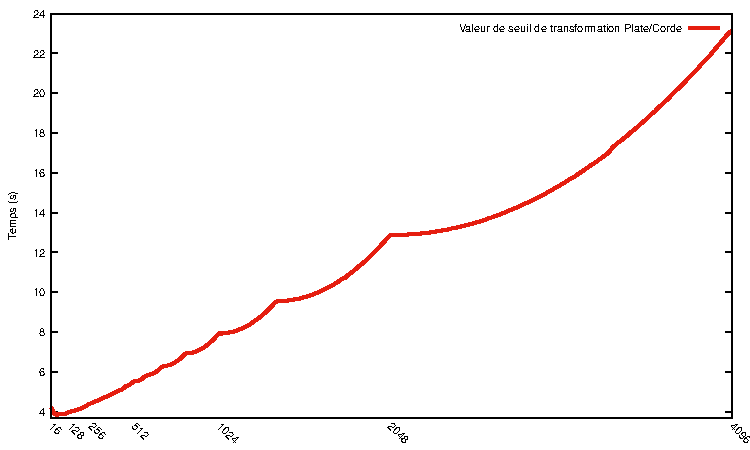
\includegraphics[]{figures/index_maxlen.pdf}
\end{figure}

Nous observons dans ce cas que la meilleure valeur de seuil, produisant des résultats minimaux est 64.
Moins que cela, le temps de parcours de la corde devient le facteur limitant, et plus que cela, le temps augmente du
fait du parcours de la chaîne plate en temps linéaire.

Les résultats sont disponibles via le tableau~\ref{index_maxlen_dat} et la figure~\ref{index_maxlen_fig}.

\subsection{Itération}

Dans ce benchmark, nous effectuons 200k itérations sur une chaîne construite procédura-lement via
des concaténations successives en début d'exécution.

\begin{table}
	\caption{\label{iter_maxlen_dat}Temps en secondes pour 200k itérations sur une chaîne de longueur 4096, en fonction du seuil de transformation corde/plate.}
	\centering
	$\begin{array}{ *{10}{c} }
		\toprule
		& 16 & 32 & 64 & 128 & 256 & 512 & 1024 & 2048 & 4096 \\
		\midrule
		& 7.47 & 6.42 & 5.91 & 5.67 & 5.55 & 5.48 & 5.47 & 5.46 & 5.3\\
		\bottomrule
	\end{array}$
\end{table}

\begin{figure}
	\caption{Temps en secondes pour 200k itérations en fonction de la longueur de la chaîne, par variation de seuil de transformation corde/plate.}
	\label{iter_maxlen_fig}
	\centering
	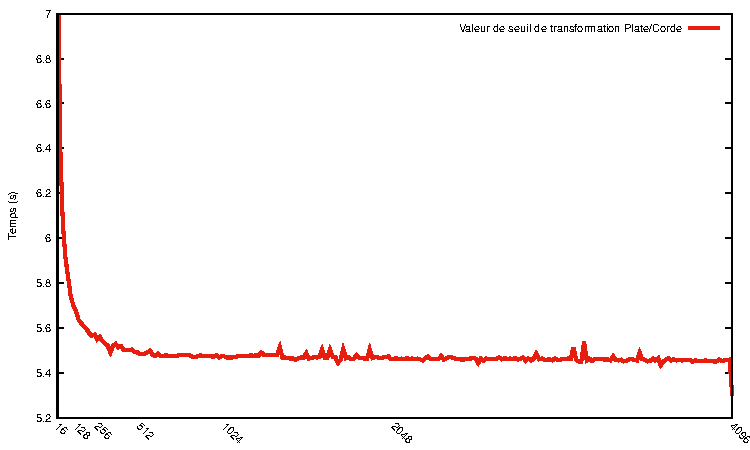
\includegraphics[]{figures/iteration_maxlen.pdf}
\end{figure}

Sans surprise ici, plus la chaîne est plate, plus l'itération est rapide, l'opération ne nécessitant pas de parcourir
de corde.
Cependant, la différence commence à être moindre à partir de 512 octets par feuille.
On notera que dans ce cas, la baisse à 4096 est due au manque total de cordes, ce qui induit un nombre plus faible d'indirections et donc une meilleure performance.

Les résultats sont disponibles via le tableau~\ref{iter_maxlen_dat} et la figure~\ref{iter_maxlen_fig}.

\subsection{Sous-chaînage}

Dans ce benchmark, nous effectuons 5M sous-chaînages successifs avec des bornes aléa-toires sur une chaîne construite
procéduralement via des concaténations successives en début d'exécution.

\begin{table}
	\caption{\label{substr_maxlen_dat}Temps en secondes pour 5M sous-chaînages en fonction de la longueur de la chaîne, par variation de seuil de transformation corde/plate.}
	\centering
	$\begin{array}{ *{10}{c} }
		\toprule
		& 16 & 32 & 64 & 128 & 256 & 512 & 1024 & 2048 & 4096\\
		\midrule
		& 38.81 & 20.06 & 10.16 & 5.40 & 3.29 & 2.06 & 1.95 & 2.49 & 3.35\\
		\bottomrule
	\end{array}$
\end{table}

\begin{figure}
	\caption{Temps en secondes pour 5M sous-chaînages en fonction de la longueur de la chaîne, par variation de seuil de transformation corde/plate.}
	\label{substr_maxlen_fig}
	\centering
	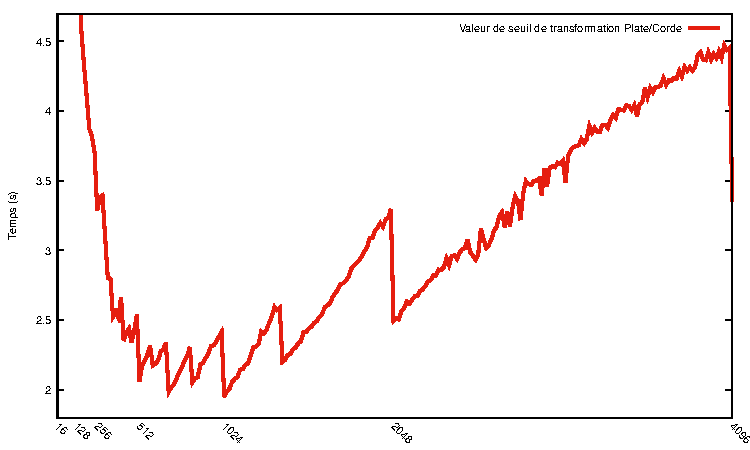
\includegraphics[]{figures/substring_maxlen.pdf}
\end{figure}

Les résultats obtenus en~\ref{substr_maxlen_dat} nous offrent des résultats intéressants,
comme le montre la figure~\ref{substr_maxlen_fig}.
En effet, le temps total de sous-chaînage dans ce cas va dépendre de la taille de seuil
de façon importante.
Une valeur de seuil trop faible entraîne le plus de surcoût dans notre cas, principalement
du a la reconstruction des noeuds de corde que produit cette approche.
Cette reconstruction entraîne la création de beaucoup d'objets éphémères, ce qui
a pour effet d'augmenter la pression sur le ramasse-miettes, et par ce fait, le
temps d'exécution augmente autant.
Cette mesure exclut le temps de ré-équilibrage des cordes, qui ferait encore augmenter
les temps d'exécution dans ce cas-ci.
On notera également qu'à partir d'une valeur de seuil de 1024, le temps recommence à
augmenter, cette fois-ci à cause du temps de parcours des feuilles, ce dernier augmentant linéairement.
Dans ce cas-ci, les meilleures valeurs de seuils à considérer sont donc comprises entre
512 et 1024.

\subsection{Conclusion}

Dans ces benchmarks, nous remarquons que dans une majorité de cas, des longueurs de feuille
aux alentours de 512 ou 1024 semblent apporter le meilleur compromis.
Cela nous conforte dans notre choix d'utiliser 512 dans notre implémentation comme seuil de passage
de chaîne plate vers corde.

\section{Étude de cas: Lecture de JSON}\label{json_perf}

JSON (JavaScript Object Notation) est un format de représentation de données
sous forme de chaînes de caractères.
Il est défini dans la RFC 7159 \cite{bray2014javascript} comme le format d'échange de
données par défaut pour le langage Javascript.
Il permet la représentation hiérarchique des données sous forme d'objets, sa grammaire
est simple et ne nécessite que peu de métadonnees pour représenter de l'information,
ce qui en fait un format efficace.
Depuis son introduction, il est devenu, à la date de redaction de ce document, l'un
des formats les plus populaires pour l'échange de données via Internet\cite{wang2011improving}.

De par son statut hégémonique, une majorité de langages de programmations populaires
modernes possèdent une implémentation d'analyseur syntaxique de JSON dans leur bibliothèque
standard. C'est le cas de Python, Ruby, Go, etc.

Cette sous-section identifie et compare les implémentations de plusieurs analyseurs syntaxiques
JSON dans differents langages: C, Go, Ruby, Python 2, Python 3 et Nit.
Deux alternatives sont présentées pour Nit: un analyseur syntaxique géneré par un outil, et un analyseur
syntaxique écrit à la main.

\subsection{Implémentations}

Les implémentations d'analyseurs syntaxiques JSON que nous étudions sont comparables au niveau de la
fonctionnalité, chacun est capable de lire une chaîne de caractères en JSON valide et de la
transformer en un objet natif du langage pour permettre son utilisation par la suite.
Les erreurs de formattage sont repérées, et renvoyées à l'utilisateur.

Les principales différences entre les implémentations viennent majoritairement de la
technique d'implémentation, du niveau d'optimisation et de la gestion du codage.

Ruby expose deux versions d'analyseur syntaxique JSON: l'une implementée en Ruby pur, qui est laissée
en dehors des chiffres du fait de sa lenteur et une autre utilisant un automate déterministe
à états finis optimisé généré en C\footnote{
\url{https://github.com/ruby/ruby/tree/c4fdfabcc8ea3f6186d1560f7756211fce125be3/ext/json/parser}.}
directement par un outil externe: Ragel \cite{ragel}.

Python possède également deux versions d'analyseur syntaxique JSON dans sa bibliotheque standard,
toutes deux implementées dans l'engin de référence du langage, \texttt{cpython}.
L'une est implémentée de facon efficace en C\footnote{\url{https://github.com/python/cpython/blob/master/Modules/_json.c}.}.
La seconde est en Python pur\footnote{\url{https://github.com/python/cpython/blob/master/Lib/json/decoder.py}.},
et sera automatiquement utilisée en cas de non-disponibilité de l'analyseur syntaxique C.
Notons que dans le cas de Python, nous faisons une différence entre la version 2 et la version
3 du langage et de l'engin d'éxécution à cause notamment de la différence de manipulation
des chaînes de caractères entre les deux versions \cite{PEP393}.

C n'a pas d'analyseur syntaxique JSON de référence, essentiellement car la bibliothèque standard
de C est assez primitive, les fonctionnalités sont souvent ajoutées via des surcouches externes.
Nous prendrons ici comme référence l'analyseur syntaxique \texttt{ujson4c}\footnote{Disponible ici \url{https://github.com/esnme/ujson4c}.}.

Go quant à lui offre un analyseur syntaxique JSON écrit complètement à la main et disponible
dans sa bibliothèque standard\footnote{\url{https://golang.org/src/encoding/json/decode.go}.}.

Pour finir, Nit expose deux implémentations d'analyseurs syntaxiques JSON.
L'un généré par NitCC\footnote{NitCC est un générateur d'analyseurs lexicaux et syntaxiques à partir d'un fichier de grammaire.},
qui produit un ensemble d'analyseurs lexicaux et syntaxiques complet pour la grammaire
de JSON. Il produit un AST\footnote{Abstract Syntax Tree, un arbre organisant hiérarchiquement les
entités d'un texte.} intermédiaire lors du parsing, ce qui en fait un analyseur syntaxique inefficace.
À cause de cela, il est mentionné, mais pas inclus dans les résultats.
Un deuxième analyseur syntaxique est une implémentation de machine à états finis en Nit pur.
Deux programmes clients de cet analyseur syntaxique sont mis à l'épreuve: l'un utilisant un mélange de cordes et
de chaînes plates, et un deuxième comptant seulement des chaînes plates.
Tous prennent en compte Unicode dans leurs routines de chaînes de caractères.

\subsection{Protocole d'expérimentation}

Les analyseurs syntaxiques sont chacun lancés sur des fichiers d'une longueur variable et avec des contenus plus ou
moins complexes.
Chaque fichier de la suite est codé en UTF-8.

\begin{enumerate}
	\item Un premier fichier\footnote{Disponible via \url{https://edg.epa.gov/data.json}.} de 6.6 Mio contenant du texte ASCII, copié 10 fois dans un tableau JSON pour un fichier de 66 Mio au total - Gov
	\item Un deuxième fichier\footnote{Disponible via \url{https://raw.githubusercontent.com/miloyip/nativejson-benchmark/master/data/twitter.json}.} de 65 kio contenant des caractères japonais, copié 200 fois dans un tableau JSON, pour un fichier de 60 Mio au total - Twitter
	\item Un troisième fichier\footnote{Disponible via \url{https://github.com/seductiveapps/largeJSON/blob/master/100mb.json?raw=true}.} de 100 Mio contenant beaucoup de caractères echappés sous la forme \textbackslash uXXXX - Large
	\item Un dernier fichier\footnote{Disponible via \url{http://mtgjson.com/json/AllSets-x.json}.} de 40 Mio contenant des caractères Unicode et ASCII - Magic
\end{enumerate}

Chaque analyseur syntaxique lit et analyse l'entrée pour créer des objets natifs au langage cible.
Chaque benchmark est exécuté 5 fois sur le fichier, et la moyenne du temps est retenue comme donnée de base, les
temps minimum et maximum sont gardés et représentés dans le graphique final.

\subsection{Résultats et discussion}

Parmi les analyseurs syntaxiques étudiés, sans surprise, la bibliotheque C \texttt{ujson4c} est la plus efficace.
En s'affranchissant de la sémantique d'Unicode quant à l'accès à un caractère et en effectuant des comparaisons
efficaces lors de la recherche d'échappements (switchs, accès à des tables pré-calculées), il est entre 4 et 5
fois plus rapide que l'implémentation Python 3.

Python 3 est la deuxième implémentation en termes d'efficacité, suivie par Python 2.
Le fait que l'analyseur syntaxique soit écrit directement en C est une aide significative dans ce cas-ci.
Notons que la différence entre Python 2 et Python 3 vient majoritairement de l'introduction de PEP-393, Python
2 perdant effectivement une partie du temps alloué à la transformation de la chaîne entrée en chaîne Unicode
Python.

\begin{table}
	\caption{\label{JSON_parse_time}Temps de parsing de fichiers JSON en fonction du langage}
	\centering
	$\begin{array}{ *{8}{c} }
		\toprule
		 & C & Python 3 & Python 2 & Go & Nit - Cordes & Nit + Cordes & Ruby \\
		\midrule
		Gov & 0.11 & 0.55 & 1.00 & 1.15 & 1.14 & 1.30 & 1.33\\
		Twitter & 0.11 & 0.7 & 1.10 & 1.12 & 1.14 & 1.24 & 1.29\\
		Large & 0.27 & 1.23 & 1.7 & 2.96 & 3.25 & 3.44 & 3.75\\
		Magic & 0.13 & 0.87 & 1.58 & 1.40 & 1.37 & 1.45 & 2.94\\
		\bottomrule
	\end{array}$
\end{table}

\begin{figure}
	\caption{Parsing JSON par langage}
	\label{jsonparse}
	\centering
	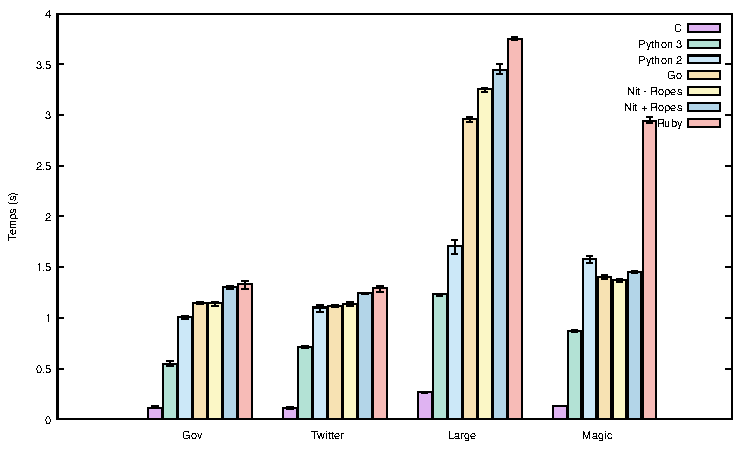
\includegraphics[]{figures/parse_json.pdf}
\end{figure}

Go est 4$^{e}$ en termes d'efficacité avec son implémentation native d'analyseur syntaxique JSON.
L'implementation Nit occupe la place qui suit, avec des résultats proches de Go. Les résultats sont
cohérents du fait de la similarité des implémentations.
En Nit, la majorité du temps est passée dans les routines de décodage de chaînes de caractères qui,
à cause d'UTF-8, augmentent le temps passé dans les accès indexés.
Un ralentissement est observé en Nit dans la version utilisant des cordes (identifiée dans le tableau~\ref{JSON_parse_time}
comme \texttt{Nit + Cordes}), cela s'explique par les performances
réduites des cordes en itération et sous-chaînage, dans un cadre où le programme les utilise intensivement, mais où
peu, voire aucune concaténation, ni accès indexé aléatoire ne sont effectués.
On notera cependant que le ralentissement observé reste du domaine de l'acceptable dans la mesure où il reste sous les
8\%, à l'exception de Gov, où il approche 15\% de différence.
Nous attribuons ce changement au fait que Gov est un fichier JSON entièrement en ASCII, sans caractères échappés,
ce qui permet aux optimisations des chaînes plates dans ce cas particulier de briller.
Ruby est en dernière place de ce comparatif, et ce malgré son implémentation C efficace.

La version NitCC, qui n'a pas été retenue pour ce comparatif, est plus lente que
la version Ruby avec un analyseur syntaxique C.
Son temps pour le fichier \texttt{Gov} est de 3.957 s, plus lente d'un facteur superieur à
2 par rapport à la version Ruby/C.
Le temps de l'analyseur syntaxique Ruby en version ruby-pure est, pour le même fichier de 7.805 s, soit près de 6 fois plus
lente que son équivalent optimisé.

\section{Étude de cas: Analyse syntaxique de documents CSV}

CSV, à l'instar de JSON, est un format de stockage de données textuelles sous forme de table.
Il est par exemple utilisé pour stocker de façon portable des données issues de tableurs comme
Microsoft Excel ou Libre Office Calc entre autres.

Il s'agit d'un format ancien, pas nécessairement en tant que fichier de données, mais comme représentation
simple de données, tel que représenté en IBM Fortran \cite{ibmfortran74} via les \texttt{FORMAT statements}.
Depuis, le format a été utilisé par un nombre conséquent de programmes et utilisateurs pour
échanger des données.
Une tentative de normalisation a été effectuée en 2005 par le biais de la RFC 4180 \cite{rfccsv}.
Cette dernière se base sur les trois principes suivants:

\begin{enumerate}
	\item Les séparateurs sont définis comme le caractère virgule (,)
	\item Les fin de lignes sont signalées par la séquence de caractères CRLF (\textbackslash r \textbackslash n)
	\item Les séquences contenant soit un séparateur, soit une fin de ligne, soit un caractère d'échappement, doivent être échappées via un caractère d'échappement ("). Ceux-ci sont doublés lorsque présents dans la chaîne échappée.
\end{enumerate}

Cette section vise à comparer plusieurs implémentations d'analyseurs syntaxiques CSV dans plusieurs langages,
sur de larges fichiers CSV.
Nous allons comparer ici les implémentations de la bibliothèque standard de Python, Ruby, Nit et Go.
Nous allons également comparer l'implémentation Java d'Apache, via le package Apache Commons
\footnote{Disponible à \url{http://apache.mirror.gtcomm.net//commons/csv/binaries/commons-csv-1.3-bin.zip}}, dans sa version 1.3.
En ce qui concerne Python, nous allons également mesurer la performance de l'analyseur de la bibliothèque
Pandas, basée sur NumPy.

\subsection{Implémentations}

A l'instar du protocole de test pour JSON, toutes les bibliothèques que nous comparons offrent des
fonctionnalités similaires.
Chaque bibliothèque aura pour but lors du test de lire un fichier CSV et de le transformer en une structure
tabulaire utilisable dans un programme écrit dans le langage cible.

Des différences seront à noter en ce qui concerne l'API de certains cependant. Python - Pandas, Nit, Go et Ruby
fonctionnent via une approche globale.
C'est à dire qu'a partir d'un fichier ou d'une chaîne de caractère, ils sont
capables de produire un tableau contenant l'ensemble des données du document en un seul appel de fonction.
Les approches suvies par Java - Apache Commons et Python - Standard, sont elles orientées sur un mécanisme
d'itérateur.
Il est donc nécessaire dans leur cas de lire le document ligne par ligne pour en stocker son contenu dans une
table.
Cette opération possède le désavantage de produire plus d'appels de fonctions, possiblement polymorphes,
ce qui induit nécessairement un ralentissement par rapport à une approche globale.

\subsection{Protocole d'expérimentation}

Chaque analyseur syntaxique sera lancé sur des fichiers contenant 1 million de lignes, plus une
ligne d'entête.
Deux fichiers générés via un outil écrit en Nit seront considérés pour cette étude:

\begin{enumerate}
	\item \texttt{1M lignes ASCII}: Un fichier contenant 1 million de lignes de données, chacune contenant 10 éléments d'une longueur aléatoire comprise entre 1 et 15 caractères \texttt{a} ainsi que des caractères nécessitant l'échappement de façon aléatoire.
	\item \texttt{1M lignes UTF-8}: Un fichier contenant 1 million de lignes de données, chacune contenant 10 éléments d'une longueur aléatoire comprise entre 1 et 15 caractères \texttt{à} ainsi que des caractères nécessitant l'échappement de façon aléatoire.
\end{enumerate}

Chaque benchmark est exécuté 5 fois sur le fichier, la moyenne du temps utilisateur est retenue comme donnée de base.
Les temps minimum et maximum sont égalements gardés pour mesurer la variabilité du test.

\subsection{Résultats et discussion}

\begin{table}
	\caption{\label{csv_numbers}Temps de parsing de fichiers CSV en fonction du langage}
	\centering
	$\begin{array}{ *{10}{c} }
		\toprule
		& \rotatebox[]{65}{Ruby} & \rotatebox[]{65}{Java} & \rotatebox[]{65}{Go} & \rotatebox[]{65}{Python2} & \rotatebox[]{65}{Python3} & \rotatebox[]{65}{Nit-Cordes} & \rotatebox[]{65}{Nit+Cordes} & \rotatebox[]{65}{Pandas2} & \rotatebox[]{65}{Pandas3}\\
		\midrule
		ASCII & 67.33 & 10.28 & 3.02 & 2.77 & 3.38 & 1.59 & 1.92 & 1.08 & 1.11\\
		Unicode & 70.15 & 10.59 & 3.79 & 2.96 & 3.67 & 3.24 & 3.65 & 1.25 & 1.3\\
		\bottomrule
	\end{array}$
\end{table}


Parmi les analyseurs étudiés, Python - Pandas est le plus efficace.
Sa rapidité vient du fait que la bibliothèque est principalement écrite en C et optimisée autant
que possible.
Les sémantiques d'accès aux caractères imposées par Unicode ne s'appliquent pas à leur analyseur, et la majorité
du code étant écrite et compilée avec les fanions d'optimisation maximum font de lui le plus rapide.

Ensuite, nous avons l'implémentation Nit, un parseur écrit à la main en Nit pur.
L'analyseur respecte les sémantiques d'Unicode pour l'accès aux caractères et les manipulations sur le contenu
d'une chaîne.
Un effort particulier a été apporté pour assurer une performance optimale dans le cas d'une bibliothèque écrite
en Nit pur.
La version utilisant les cordes est, à l'instar de l'analyseur JSON, plus lente que la version ne les utilisant pas,
dans une marge acceptable (entre 5 et 10\%).
On notera que le fichier contenant des chaînes Unicode est beaucoup plus lente que celle contenant des chaînes uniquement
ASCII.
Cette différence s'explique du fait des optimisations effectuées dans la bibliothèque du langage pour accélérer le traitement
des chaînes ASCII, statistiquement plus fréquentes.

Les implémentations Go et Python - Standard offrent une performance similaire, les deux étant écrits dans des langages
proches de la machine pour en améliorer la performance.
On notera cependant que Python 2 est légèrement plus rapide que Python 3 dans ce cas-ci, ce dernier s'affranchissant
des préoccupations d'Unicode et ne nécessitant pas de travail préalable pour la construction d'une chaîne de caractères.
Dans ce cas particulier, PEP-393 provoque un ralentissement de l'implémentation Python.

Java est avant dernier dans ce test, avec un temps près de 3 fois plus lent que les implémentations Go et
Python - Standard.
On notera que dans le cas de Java, le fichier comportant de l'Unicode ne provoque pas de ralentissement lors
de la phase d'analyse.
Ce comportement s'explique du fait de l'étape de conversion du contenu du fichier vers UTF-16.
Une fois la conversion effectuée, la lecture des caractères s'effectue en temps constant dans ce cas.

Ruby, avec une implémentation en pur Ruby, est la plus lente de notre comparatif, près de 7 fois plus
lente que l'implémentation Java.

L'ensemble des résultats sont disponibles via le tableau \ref{csv_numbers} et la figure \ref{csv_graph}.

\begin{figure}
	\caption{Parsing CSV par langage}
	\label{csv_graph}
	\centering
	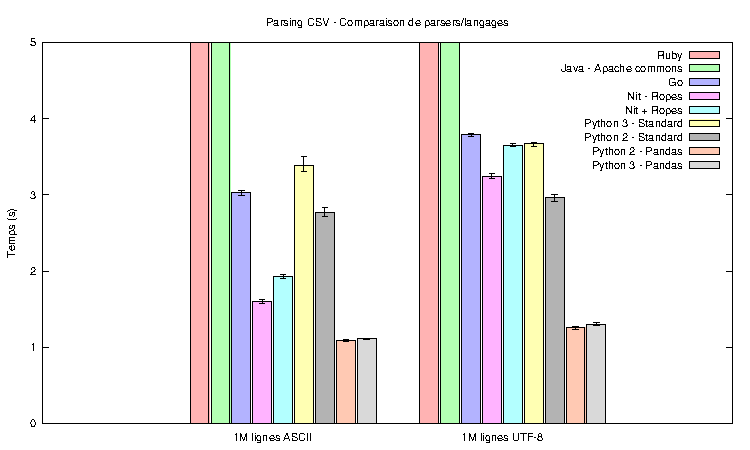
\includegraphics[]{figures/csv_bench.pdf}
\end{figure}

\section{Étude de cas: Le compilateur Nit, nitc}

Le compilateur est un des programmes les plus importants de la base de code de Nit.
Puisqu'il s'agit d'un programme indispensable à tout développeur Nit, il se doit
d'être le plus performant possible.
Dans la mesure où une grande partie de son travail consiste à lire, traiter et générer
du texte, il s'agit d'un cas très pertinent pour cette étude.

Nous allons uniquement comparer des variations de techniques de gestion des chaînes
de caractères et exposer le temps moyen d'exécution sur 5 exécutions du compilateur
se compilant lui-même.
Afin d'assurer plus de stabilité dans les chiffres et de minimiser l'impact de la
compilation du C généré par `nitc`, nous allons pré-compiler 4 fois le compilateur
avec lui-même avant d'effectuer la mesure.

Nous allons étudier l'impact sur deux techniques de compilation de nitc, en compilation
séparée et en compilation semi-globale.
Cette dernière effectuant plus d'optimisations en supposant une connaissance globale
du programme compilé; elle effectuera plus
d'\texttt{inlining}\footnote{Extension d'une méthode directement dans le code généré, évitant le coût de l'appel.}
de méthodes et remplacera
certains appels polymorphes par des appels monomorphes, resultant en un code globalement
plus efficace.

\subsection{Résultats et discussion}

Le tableau \ref{nitc_time} et les figures \ref{nitc_sep} et \ref{nitc_sg_vars} présentent les résultats de
la compilation de nitc avec nitc, en compilation séparée et semi-globale.
Comme attendu, la version semi-globale est plus rapide que la version
séparée.

\begin{table}
	\caption{\label{nitc_time}Temps d'exécution de `nitc src/nitc.nit` en fonction des variations d'implémentation de chaînes de caractères}
	\centering
	$\begin{array}{ *{6}{c} }
		\toprule
		 & Cordes + Plates & Plates & Cordes & Lineaire & Buffered \\
		\midrule
		separate & 3.9 & 4.11 & 4.33 & 3.86 & 4.10\\
		semi-global & 3.75 & 3.95 & 4.13 & 3.73 & 4.06\\
		\bottomrule
	\end{array}$
\end{table}

\begin{figure}
	\caption{Temps d'exécution de la commande `nitc src/nitc.nit --separate` en fonction des variations d'implémentation de chaînes de caractères}
	\label{nitc_sep}
	\centering
	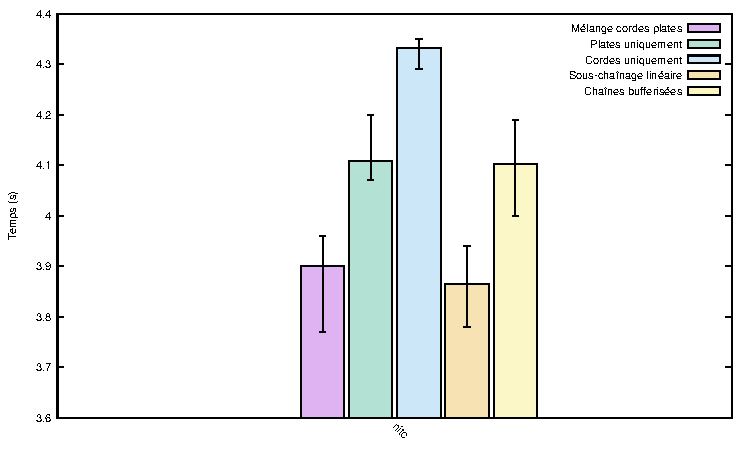
\includegraphics[]{figures/nitc_separate_vars.pdf}
\end{figure}

\begin{figure}
	\caption{Temps d'exécution de la commande `nitc src/nitc.nit --semi-global` en fonction des variations d'implémentation de chaînes de caractères}
	\label{nitc_sg_vars}
	\centering
	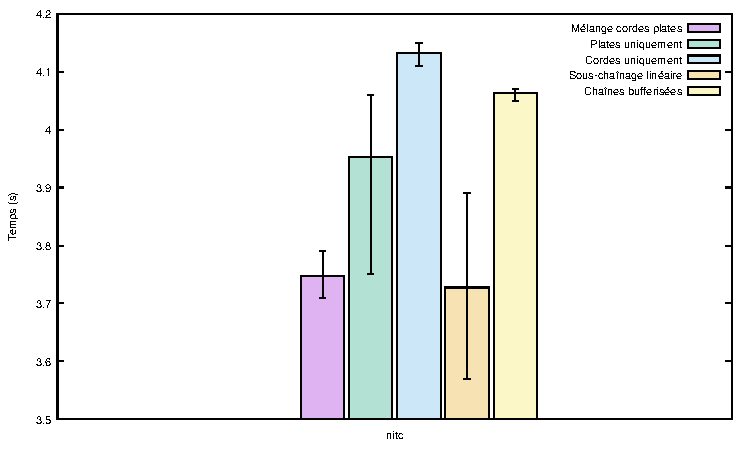
\includegraphics[]{figures/nitc_semi-global_vars.pdf}
\end{figure}

La version de base, celle qui est présentement implémentée et utilisée dans la bibliothèque
standard de Nit est la version utilisant le mélange de cordes et de chaînes plates.

Parmi les variations étudiées, nous remarquons que la variation utilisant une opération de
sous-chaînage en temps linéaire est plus rapide que ses équivalentes utilisant le partage
de chaînes.
Nous attribuons cet avantage à la structure plus légère de la chaîne produite, ce qui permet
à l'ensemble des opérations subséquentes de s'effectuer plus rapidement.
Le surcoût induit par la réallocation et la copie de la chaîne est moindre comparé
aux bénéfices de temps sur le reste des opérations.

Les chaînes sur-allouantes ne présentent pas de véritable gain dans cette configuration et font
perdre du temps, cette perte peut être imputée en grande partie aux indirections supplémentaires
et à l'alourdissement de la structure.
Dans le cas du compilateur, il est à noter également que les concaténations multiples sont rares,
car optimisées à l'aide de \texttt{Buffers}.
Il est donc normal dans ce cas de figure que la solution n'apporte pas de réel bénéfice.
Il s'agit cependant du cas le plus fréquent dans les applications optimisées pour ce genre
d'utilisations.

Les cordes systématiques sont peu pertinentes dans la mesure où les concaténations sont
réalisées via des buffers dans une majorité de cas, mais où les accès et itérations sont
fréquents, ce qui a pour conséquence de ralentir l'exécution.

Les chaînes uniquement plates sont elles aussi perdantes dans ce cas de figure, le principal
défaut de cette approche étant que le travail de parcours de chaîne est onéreux lorsqu'effectué
loin du cache.
Ce cas-ci est rare, mais présent dans le compilateur lors de la production tardive d'une sous-chaîne
pour récupérer le contenu d'un jeton lors de phases d'analyses subséquentes.
La limite de la taille des feuilles et l'accès en O(log(n)) sont ici bénéfiques.

\subsection{Variation du seuil de concaténation}

Nous incluons le compilateur dans nos benchmarks de vérification du seuil par défaut des transformations
de chaines plates vers cordes.
Le modus operandi ici est similaire à celui utilisé dans les micro-benchmarks en \ref{rope_flat_thres_bench},
en faisant varier le seuil de transformation sur des puissances de 2, de 16 à 4096.

\begin{table}
	\caption{\label{nitc_time_maxlen}Temps d'exécution de `nitc src/nitc.nit` en fonction du seuil de conversion plate/corde}
	\centering
	$\begin{array}{ *{10}{c} }
		\toprule
		& 16 & 32 & 64 & 128 & 256 & 512 & 1024 & 2048 & 4096 \\
		\midrule
		separate & 4.23 & 3.93 & 3.94 & 3.88 & 3.91 & 3.95 & 3.95 & 3.9 & 3.93\\
		semi-global & 4.05 & 3.72 & 3.77 & 3.75 & 3.70 & 3.74 & 3.73 & 3.72 & 3.76\\
		\bottomrule
	\end{array}$
\end{table}

\begin{figure}
	\caption{Temps d'exécution de la commande `nitc src/nitc.nit` en fonction du seuil de conversion plate/corde}
	\label{nitc_sep_maxlen}
	\centering
	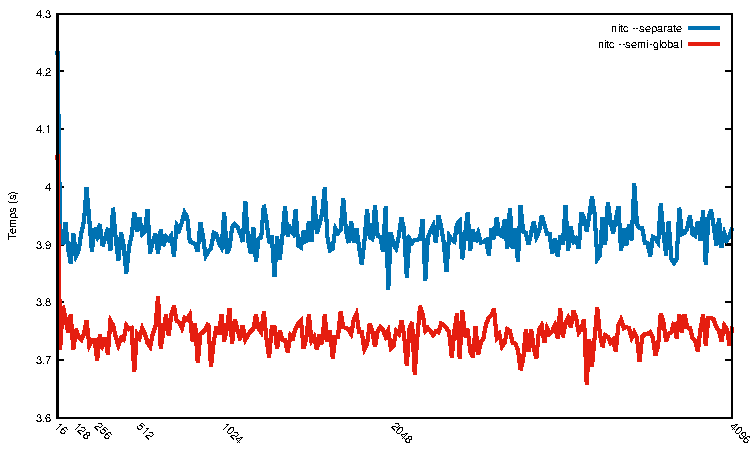
\includegraphics[]{figures/nitc_separate_maxlen.pdf}
\end{figure}

Nous observons cependant peu de différences dépendamment directement du seuil, pourvu que celui-ci
soit au moins de 32.
Les résultats sont disponibles via le tableau~\ref{nitc_time_maxlen} et la figure~\ref{nitc_sep_maxlen}.

\section{Étude de cas: nitlight}

Nitlight est un outil écrit en Nit base sur la chaîne d'outils dérivée du
compilateur.
Il sert à produire des fichiers HTML contenant le code source d'un fichier
coloré, avec des liens sémantiques vers la documentation et les entités
comprises dans le code.

Par sa nature d'analyseur et producteur de chaînes, ce dernier est intéressant
pour juger de la performance de notre implémentation, et plus particulièrement
pour étudier les différents seuils de transformation de chaîne plate vers corde.

Ce benchmark va lancer nitlight pour compiler les fichiers HTML liés au compilateur
ainsi que toutes ses dépendances.
Le modus operandi pour la mesure de la performance est identique à celui
utilisé précédemment.

\subsection{Résultats et discussion}

Comme dans le cas du compilateur, la variation du seuil de transformation
ne s'avère pas avoir beaucoup d'effet passé un seuil minimal de 64.
En effet, passé ce seuil, la durée d'une exécution reste stable, avec une variation de +/- 0.1s.

\begin{table}
	\caption{\label{nitlight_time_maxlen}Temps d'exécution de `nitlight --full -d out\_dir nitc.nit` en fonction du seuil de conversion plate/corde}
	\centering
	$\begin{array}{ *{10}{c} }
		\toprule
		& 16 & 32 & 64 & 128 & 256 & 512 & 1024 & 2048 & 4096\\
		\midrule
		separate & 6.45 & 6.42 & 5.91 & 5.86 & 5.83 & 5.97 & 5.94 & 5.98 & 5.83\\
		semi-global & 5.74 & 5.70 & 5.37 & 5.31 & 5.32 & 5.37 & 5.31 & 5.32 & 5.35\\
		\bottomrule
	\end{array}$
\end{table}

\begin{figure}
	\caption{Temps d'exécution de la commande `nitlight --full -d out\_dir nitc.nit` en fonction du seuil de conversion plate/corde}
	\label{nitlight_sep_maxlen}
	\centering
	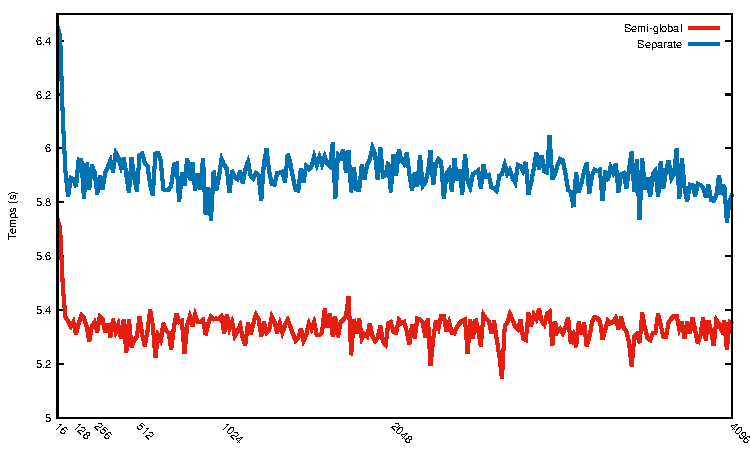
\includegraphics[]{figures/nitlight.pdf}
\end{figure}

Les résultats sont disponibles via le tableau~\ref{nitlight_time_maxlen} et la figure~\ref{nitlight_sep_maxlen}.

\section{Conclusion}

Ce chapitre présente une suite de programmes de mesure de la performance, constituant une validation de notre solution.
En effet, en mélangeant les cordes aux chaînes plates, et en utilisant une stratégie efficace pour la production de ces
dernières, nous mitigeons les cas dégénératifs exposés par les deux structures, et pouvons utiliser l'une représentation
ou l'autre de façon complètement transparente.

Des optimisations restent cependant à étudier pour limiter encore les problèmes que posent une
structure arborescente pour les chaînes dans les cas courants, tels que nous pouvons voir dans 
l'analyseur syntaxique JSON.
